\documentclass[11pt,a4paper]{article}

\usepackage[utf8]{inputenc}
\usepackage[T1]{fontenc}
\usepackage[brazilian]{babel}
\usepackage{amsmath,amssymb}
\usepackage{geometry}
\usepackage{indentfirst}
\usepackage[hidelinks]{hyperref}
\usepackage{titlesec}
\usepackage{enumitem}
\usepackage{graphicx}
\usepackage{booktabs}
\usepackage{caption}
\usepackage{subcaption}
\usepackage{microtype}

\geometry{a4paper, top=1.70cm, bottom=1.70cm, left=1.80cm, right=1.80cm}
\linespread{0.96}

\titlespacing*{\section}{0pt}{1.0ex plus .2ex minus .2ex}{0.4ex plus .1ex}
\titlespacing*{\subsection}{0pt}{0.7ex plus .2ex minus .1ex}{0.3ex plus .1ex}
\setlist{noitemsep, topsep=1pt, parsep=0pt, partopsep=0pt}

\setlength{\abovedisplayskip}{2.5pt plus 1pt minus 1pt}
\setlength{\belowdisplayskip}{2.5pt plus 1pt minus 1pt}

\title{\textbf{\large Redes Neurais Informadas por Física (PINNs) versus Métodos de Diferenças Finitas (ADI) na Solução da Equação do Calor 2D em Domínios Irregulares}}

% Versão anônima para submissão inicial (avaliação duplo-cega conforme Edital n.º 04/2026)
\author{
  \normalsize\textit{Autoria omitida para avaliação duplo-cega}\\[0.2em]
  \small Campus da Universidade Federal do Ceará em Quixadá
}

\date{}

\begin{document}

\maketitle

\vspace{-1.5em}
\begin{abstract}
\noindent
A modelagem numérica da condução térmica bidimensional transiente em sólidos é historicamente dominada por métodos de Diferenças Finitas, destacando-se o método de Direções Alternadas Implícitas (ADI de Peaceman-Rachford) por sua velocidade linear $\mathcal{O}(N)$ e estabilidade incondicional em malhas regulares. Contudo, em geometrias perfuradas ou com contornos curvos, o ADI perde sua estrutura matricial tridiagonal e sofre com erros de escadeamento de malha (\textit{staircasing}). Neste trabalho, investiga-se como as Redes Neurais Informadas por Física (PINNs) superam essa restrição geométrica por meio de uma formulação contínua e livre de malha. Apresenta-se a definição precisa do domínio espaço-temporal $\Omega \times (0, T]$, a física dos sumidouros térmicos circulares e as três modificações fundamentais que convertem uma rede neural tradicional em uma PINN. Em experimentos no quadrado regular, o ADI comprova sua superioridade em problemas simples (erro $\sim 10^{-5}$ em 0,04 s frente a 42 s da PINN). Por outro lado, em uma chapa complexa com três sumidouros térmicos circulares internos, a PINN demonstra expressiva flexibilidade, capturando com alta fidelidade o campo térmico transiente e as isotermas de contorno sem necessidade de geração de malha ($\mathcal{L}_{\text{total}} \sim 6{,}2 \times 10^{-5}$, erro de contorno $< 8 \times 10^{-3}$).

\vspace{0.35em}
\noindent
\textbf{Palavras-chave:} Equação do calor; Diferenças Finitas; Método ADI; PINNs; Domínios Irregulares; Redes Neurais.

\vspace{0.2em}
\noindent
\textbf{ODS:} indústria, inovação e infraestrutura.
\end{abstract}

\vspace{0.3em}
\begin{center}
\textbf{Abstract}
\end{center}
\vspace{-0.5em}
\noindent
\small\textit{Numerical modeling of transient 2D heat conduction in solid media is historically dominated by Finite Difference methods, notably the Alternating Direction Implicit scheme (Peaceman-Rachford ADI), which achieves unconditional stability and linear $\mathcal{O}(N)$ cost on regular Cartesian grids. However, in perforated or curved geometries, ADI suffers from the breakdown of its tridiagonal matrix structure and boundary staircasing errors. In this paper, we explore how Physics-Informed Neural Networks (PINNs) overcome these geometric limitations through a mesh-free continuous framework. We clearly define the space-time domain $\Omega \times (0, T]$, the physical mechanism of circular cooling sinks, and the three foundational modifications transforming a standard neural network into a PINN. In regular square benchmarks, ADI proves superior on simple setups (error $\sim 10^{-5}$ in 0.04 s vs. 42 s of PINN training). Conversely, in a complex plate containing three internal circular cooling sinks, PINNs excel in geometric adaptability, accurately resolving the transient temperature field without remeshing ($\mathcal{L}_{\text{total}} \sim 6.2 \times 10^{-5}$, boundary error $< 8 \times 10^{-3}$).}

\vspace{0.35em}
\noindent
\textbf{Keywords:} Heat equation; Finite Differences; ADI Method; PINNs; Irregular Domains; Neural Networks.

\vspace{0.2em}
\noindent
\textbf{SDG:} industry, innovation and infrastructure.
\normalsize

\section{O Problema Físico e a Definição do Domínio Espaço-Temporal}

A condução térmica transiente em uma chapa sólida bidimensional homogênea e isotrópica com difusividade térmica $\alpha > 0$ é governada pela equação diferencial parcial (EDP) parabólica:
\begin{equation}
\frac{\partial u}{\partial t} = \alpha \nabla^2 u = \alpha \left( \frac{\partial^2 u}{\partial x^2} + \frac{\partial^2 u}{\partial y^2} \right) \quad \text{em} \quad \Omega \times (0, T],
\label{eq:heat}
\end{equation}
onde a notação do domínio representa o produto cartesiano entre o espaço e o tempo:
\begin{itemize}
  \item \textbf{Domínio Espacial ($\Omega \subset \mathbb{R}^2$):} representa a região geométrica física ocupada pela chapa sólida no plano cartesiano $(x, y) \in [0, 1] \times [0, 1]$. Quando a peça contém furos ou canais internos, o domínio $\Omega$ é a área sólida restante após subtrair os orifícios $\mathcal{H}_k$:
  \begin{equation}
  \Omega = \left\{ (x, y) \in [0, 1]^2 \;\middle|\; (x - x_k)^2 + (y - y_k)^2 > r_k^2, \; \forall k \in \{1, 2, 3\} \right\};
  \end{equation}
  \item \textbf{Domínio Temporal ($(0, T] \subset \mathbb{R}$):} representa o intervalo contínuo de tempo em que a difusão ocorre, partindo do estado inicial $t = 0$ até o tempo final $T_{\text{max}} = 1{,}0$;
  \item \textbf{Cilindro Espaço-Temporal ($\Omega \times (0, T]$):} estabelece que a equação \eqref{eq:heat} deve ser satisfeita para todo ponto espacial $(x, y) \in \Omega$ em cada instante de tempo $t \in (0, T_{\text{max}}]$.
\end{itemize}

\begin{figure}[htbp]
\centering
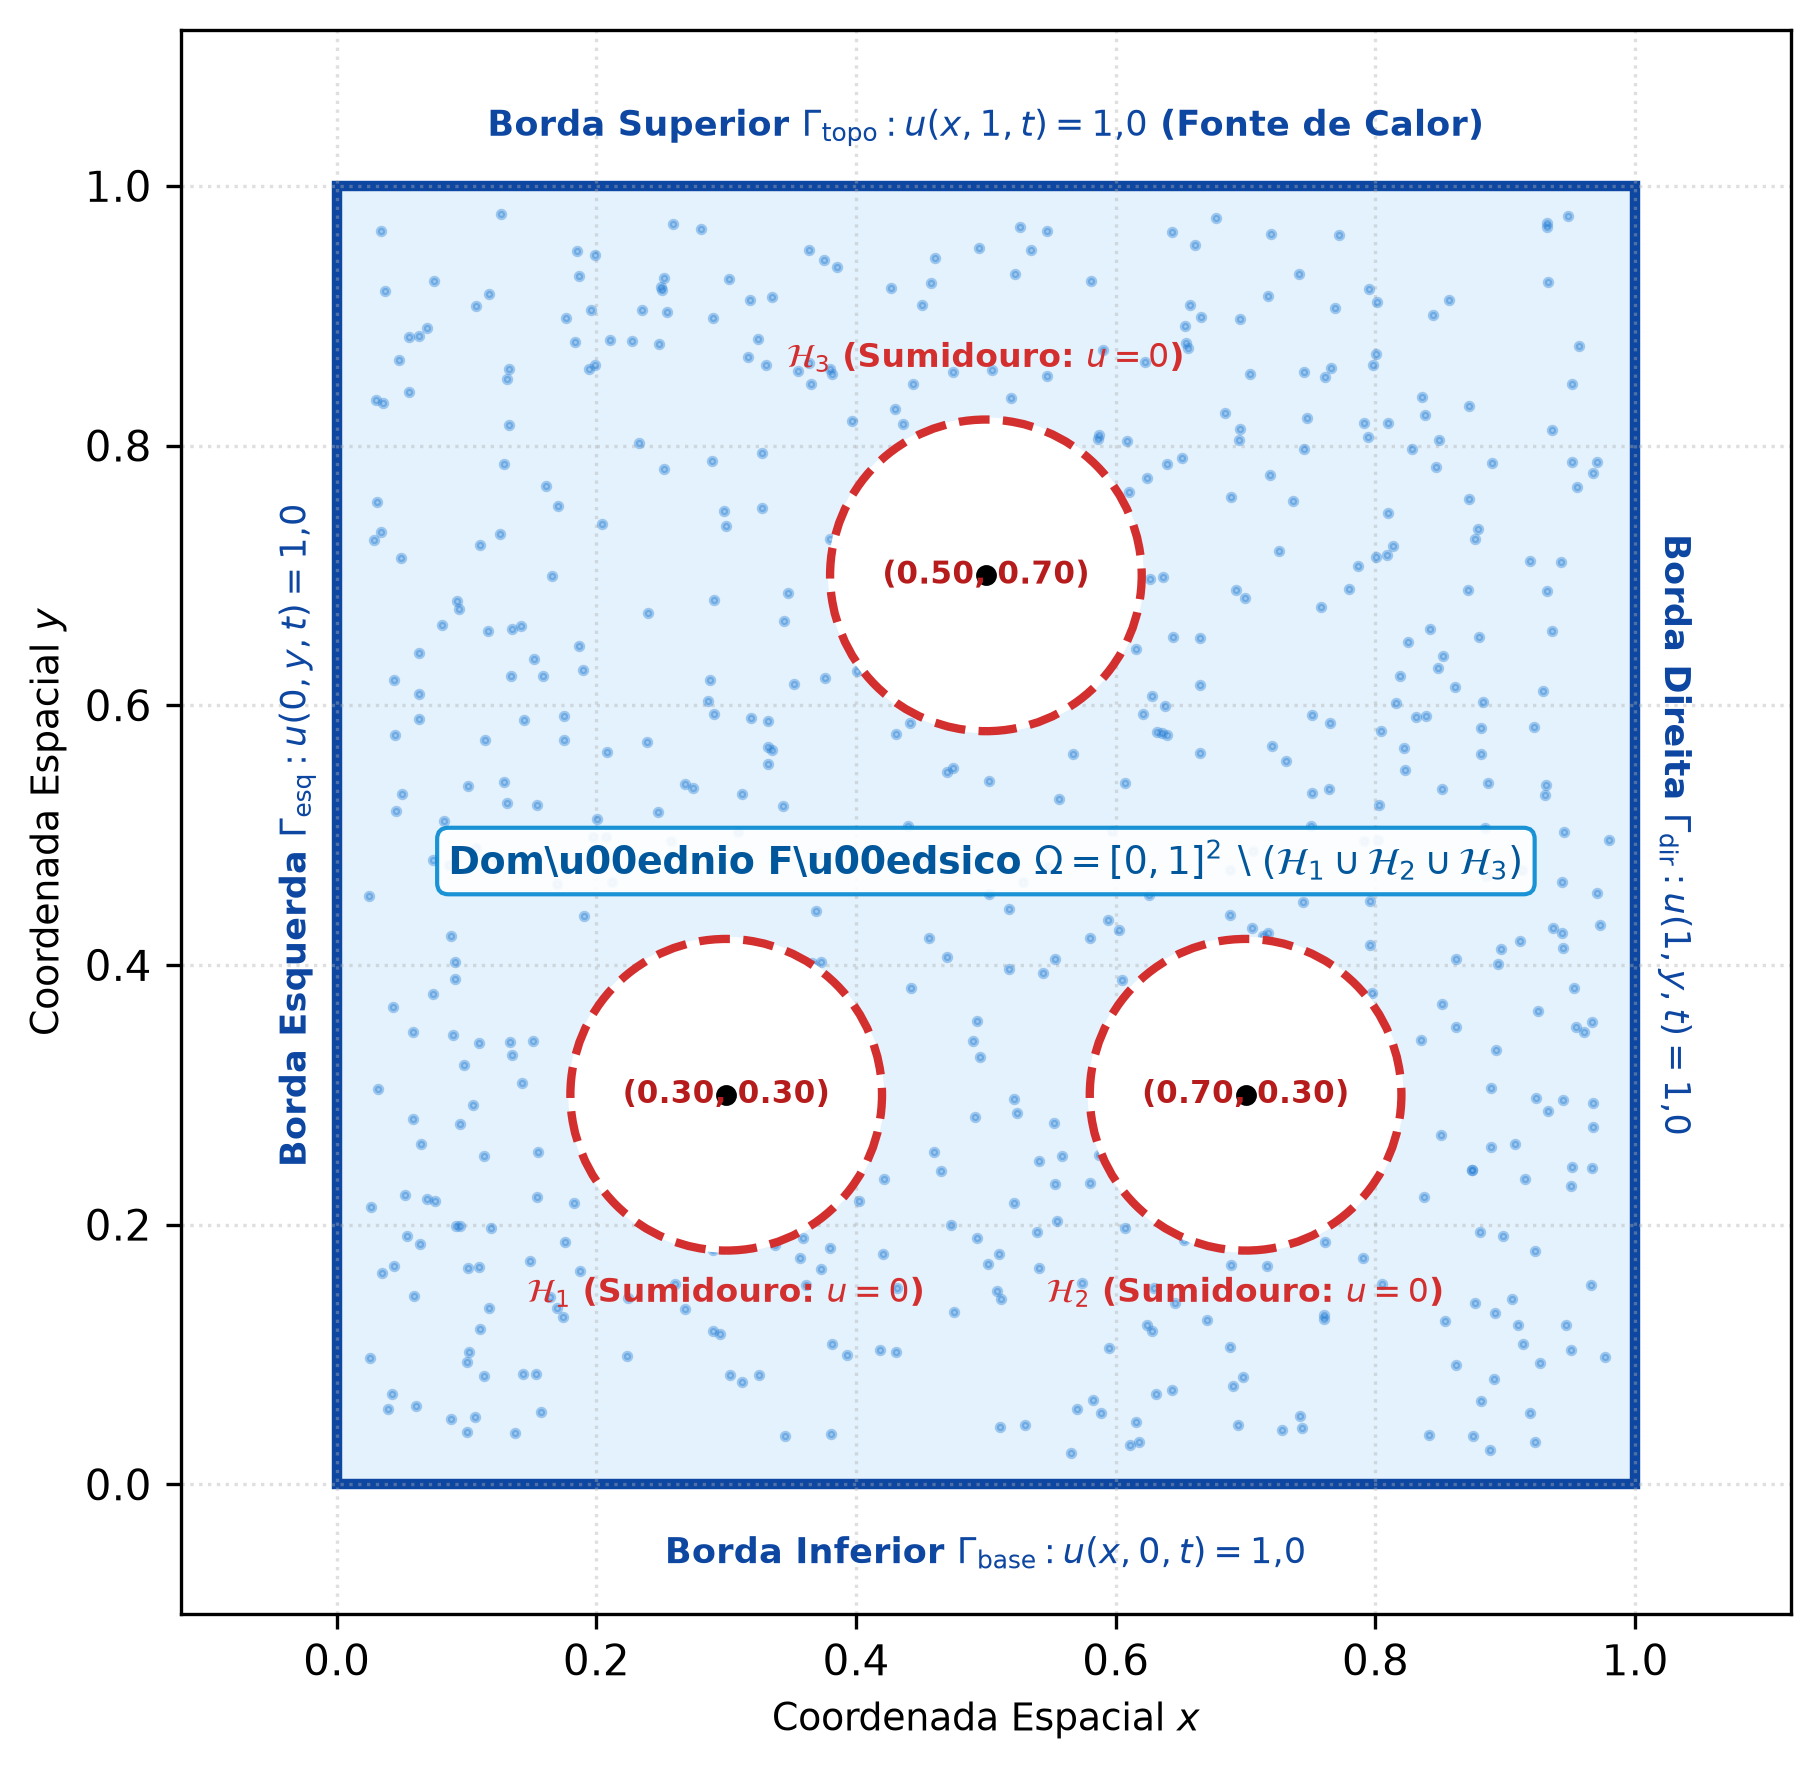
\includegraphics[width=0.62\textwidth]{figures/geometry_domain_holes.png}
\caption{Representação esquemática do domínio espacial perfurado $\Omega$: chapa quadrada $[0,1]^2$ com 4 paredes externas aquecidas ($u=1{,}0$) e 3 orifícios circulares internos mantidos a $u=0{,}0$ atuando como sumidouros térmicos de resfriamento.}
\label{fig:geometry_domain}
\end{figure}

\textbf{Física do Domínio com Três Furos Circulares:} Como ilustrado na Figura~\ref{fig:geometry_domain}, a peça analisada possui dimensões unitárias ($x \in [0,1], y \in [0,1]$) com três furos circulares de raio $r = 0{,}12$ centrados em:
\begin{equation}
\mathcal{H}_1 = (0{,}30;\, 0{,}30), \quad \mathcal{H}_2 = (0{,}70;\, 0{,}30), \quad \mathcal{H}_3 = (0{,}50;\, 0{,}70).
\end{equation}

As condições de contorno e inicial que regem o fenômeno térmico são:
\begin{enumerate}
  \item \textbf{Condição Inicial:} A chapa inicia-se inteiramente em repouso térmico a temperatura nula: $u(x, y, 0) = 0$, $\forall (x, y) \in \Omega$;
  \item \textbf{Bordas Externas ($\Gamma_{\text{ext}} = \partial [0,1]^2$):} As 4 paredes exteriores atuam como fontes de calor mantidas a $u(x, y, t) = 1{,}0$;
  \item \textbf{Bordas dos Furos ($\Gamma_{\text{int}} = \bigcup_{k=1}^3 \partial\mathcal{H}_k$):} Os três orifícios atuam como canais de resfriamento mantidos a temperatura nula ($u = 0{,}0$), drenando continuamente o calor que se propaga das bordas externas e gerando frentes de difusão com fortes gradientes isotérmicos.
\end{enumerate}

\section{O que é uma Rede Neural e o que a Transforma em uma PINN?}

\subsection{Redes Neurais Artificiais Tradicionais (MLP)}

Uma Rede Neural do tipo Perceptron Multicamadas (MLP) é um aproximador universal de funções contínuas (HORNIK et al., 1989). A rede recebe entradas numéricas $\mathbf{z}^{(0)}$ e propaga os dados através de $L$ camadas de neurônios interconectados por pesos sinápticos $W^{(l)}$ e vieses $\mathbf{b}^{(l)}$:
\begin{equation}
\mathbf{z}^{(l)} = W^{(l)} \mathbf{a}^{(l-1)} + \mathbf{b}^{(l)}, \quad \mathbf{a}^{(l)} = \sigma\left(\mathbf{z}^{(l)}\right), \quad l = 1, \dots, L,
\end{equation}
onde $\sigma(\cdot)$ é uma função de ativação não linear. No paradigma tradicional de \textit{Deep Learning} supervisionado, a rede depende de um banco de dados rotulados $\{(X_i, Y_i)\}$, ajustando seus pesos para minimizar uma perda empírica $\mathcal{L} = \frac{1}{N}\sum |\hat{Y}_i - Y_i|^2$.

\begin{figure}[htbp]
\centering
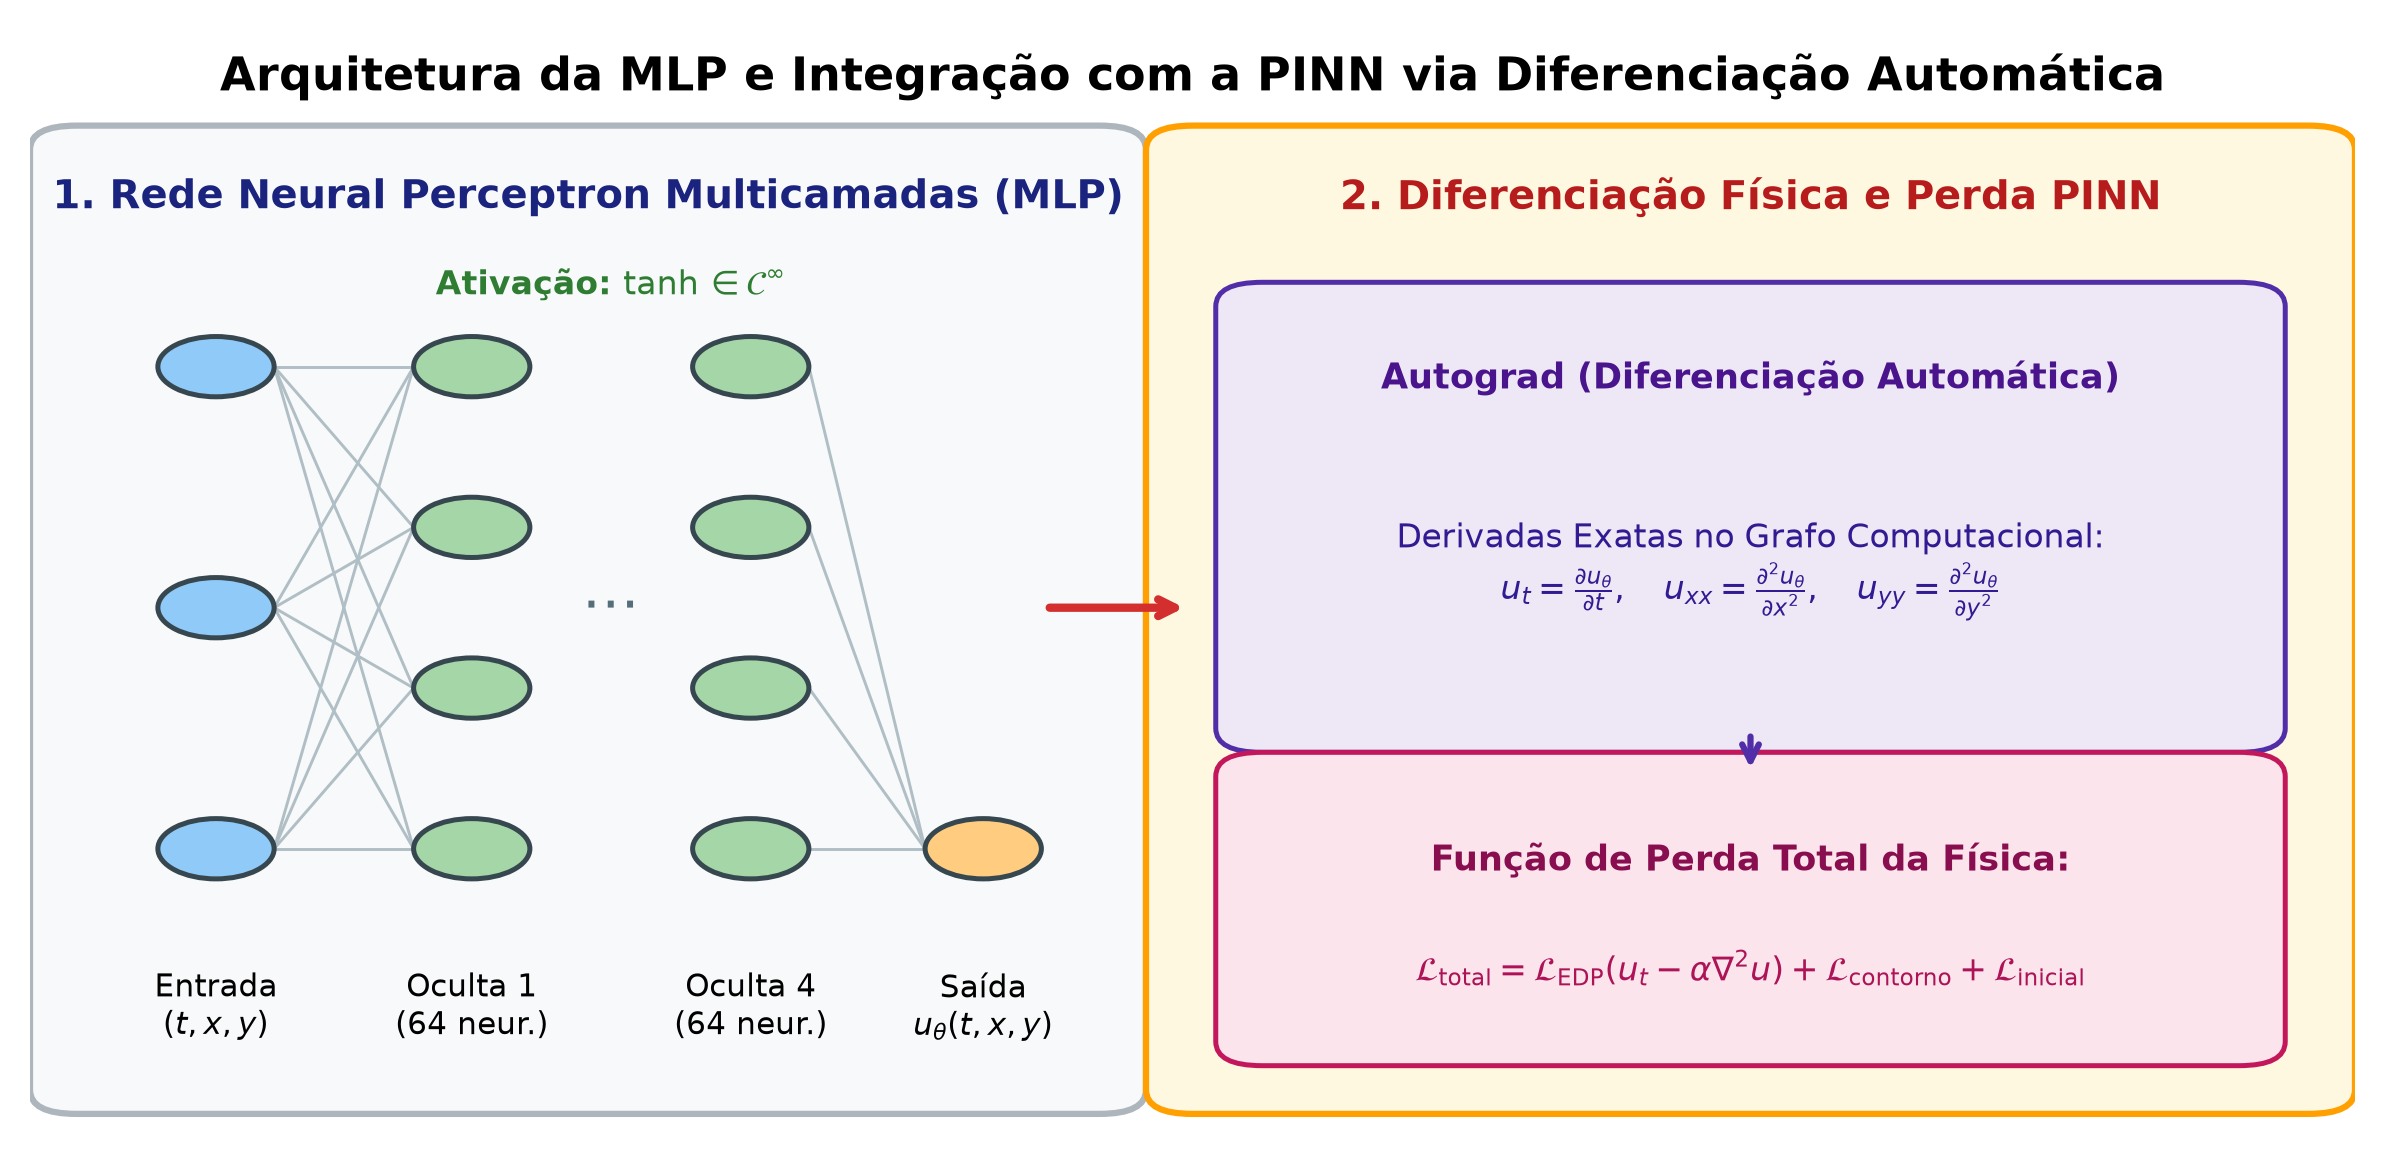
\includegraphics[width=0.88\textwidth]{figures/mlp_and_pinn_architecture.png}
\caption{Esquema da arquitetura de uma PINN: à esquerda, o Perceptron Multicamadas (MLP); à direita, o acoplamento do motor de Diferenciação Automática (Autograd) calculando derivadas exatas da EDP e formando a perda física.}
\label{fig:mlp_pinn_arch}
\end{figure}

\subsection{As 3 Modificações Fundamentais que Criam uma PINN}

Propostas por Raissi et al. (2019), as Redes Neurais Informadas por Física (\textit{Physics-Informed Neural Networks} -- PINNs) transformam o aprendizado profundo em um solucionador numérico de EDPs. Como ilustrado na Figura~\ref{fig:mlp_pinn_arch}, a transição de uma rede tradicional para uma PINN fundamenta-se em três modificações:

\begin{enumerate}[label=\textbf{\arabic*.}]
  \item \textbf{Função de Perda Baseada nas Leis da Física (Sem Rótulos Externos):} Em vez de exigir dados pré-calculados, a perda é formulada diretamente pela soma ponderada dos resíduos das equações governantes:
  \begin{equation}
  \mathcal{L}_{\text{total}}(\theta) = \lambda_{\text{pde}} \mathcal{L}_{\text{pde}} + \lambda_{\text{ic}} \mathcal{L}_{\text{ic}} + \lambda_{\text{bc}}^{\text{ext}} \mathcal{L}_{\text{bc}}^{\text{ext}} + \lambda_{\text{bc}}^{\text{furos}} \mathcal{L}_{\text{bc}}^{\text{furos}},
  \end{equation}
  onde $\mathcal{L}_{\text{pde}} = \frac{1}{N_f} \sum |u_t - \alpha(u_{xx} + u_{yy})|^2$ avalia a aderência à equação do calor no interior do domínio.

  \item \textbf{Autograd como Operador Diferencial de 2ª Ordem no Fluxo Direto:} O Autograd calcula exatamente as derivadas físicas $\frac{\partial u_\theta}{\partial t}$, $\frac{\partial^2 u_\theta}{\partial x^2}$ e $\frac{\partial^2 u_\theta}{\partial y^2}$ no fluxo direto da rede aplicando a regra da cadeia no grafo computacional, sem introduzir erros de truncamento de malha ($h^2$). Para viabilizar derivadas de 2ª ordem não nulas, a ativação deve ser suave $\mathcal{C}^\infty$ (adota-se $\tanh$), visto que ativações por partes como ReLU produzem $\nabla^2 u_\theta \equiv 0$.

  \item \textbf{Amostragem Espaço-Temporal Contínua e Livre de Malha (\textit{Collocation}):} A rede não recebe datasets estáticos, mas coordenadas contínuas $(t, x, y)$ sorteadas livremente no domínio espaço-temporal $\Omega \times [0, T]$ por amostragem de colocação. Em geometrias perfuradas, a seleção de pontos é feita por simples filtragem booleana, eliminando a necessidade de geração de malhas.
\end{enumerate}

\section{Domínios Regulares: Onde o Método ADI é Imbatível}

Para geometrias simples como o quadrado unitário sem furos $\Omega = [0, 1]^2$, o método clássico de Diferenças Finitas com Direções Alternadas Implícitas (ADI de Peaceman-Rachford) (PEACEMAN; RACHFORD, 1955; PEREIRA, 2019) fraciona o Laplaciano em dois subpassos de tamanho $\Delta t / 2$:
\begin{align}
\left( \mathcal{I} - \frac{\Delta t}{2} \alpha \partial_{xx} \right) u^{n+1/2} &= \left( \mathcal{I} + \frac{\Delta t}{2} \alpha \partial_{yy} \right) u^n, \label{eq:adi1} \\
\left( \mathcal{I} - \frac{\Delta t}{2} \alpha \partial_{yy} \right) u^{n+1} &= \left( \mathcal{I} + \frac{\Delta t}{2} \alpha \partial_{xx} \right) u^{n+1/2}. \label{eq:adi2}
\end{align}

Como as derivadas espaciais centradas em malha cartesiana regular $N_x \times N_y$ desacoplam as direções $x$ e $y$, cada subpasso resolve apenas matrizes tridiagonais via algoritmo de Thomas em tempo linear $\mathcal{O}(N_x N_y)$ (PEREIRA, 2019).

\begin{figure}[htbp]
\centering
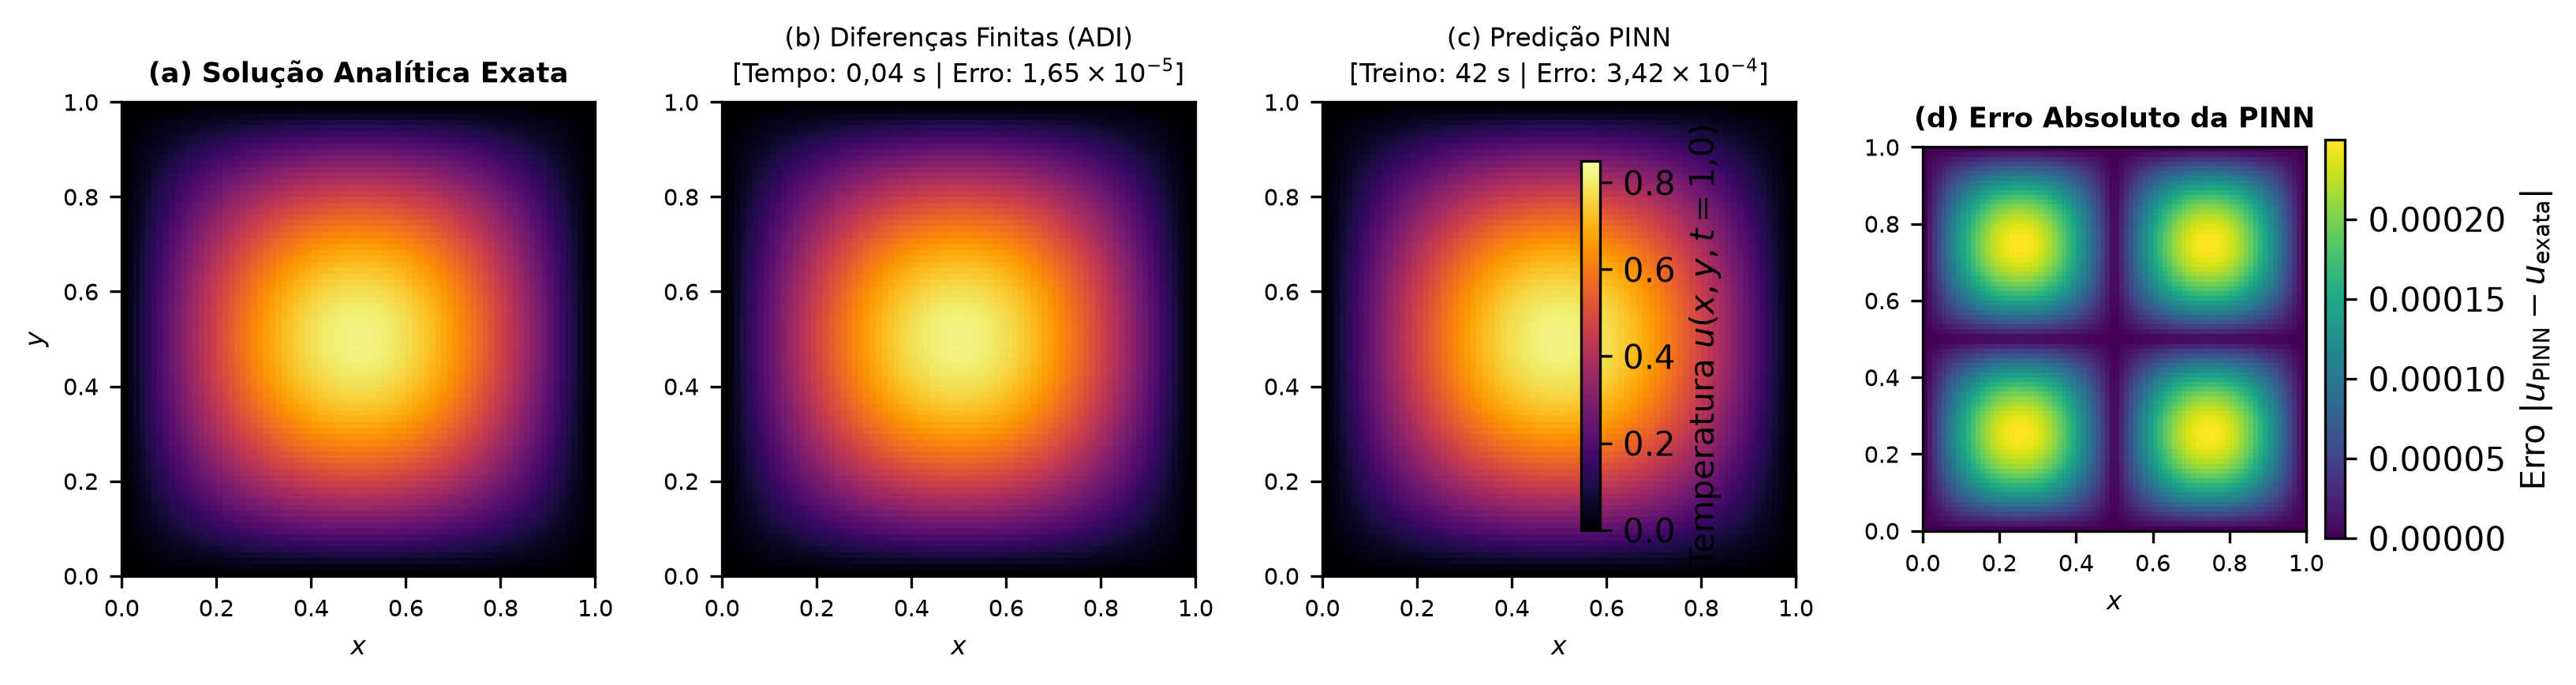
\includegraphics[width=0.95\textwidth]{figures/adi_regular_benchmark.png}
\caption{Validação canônica no quadrado regular em $t=1{,}0$: (a) Solução analítica exata; (b) Solução numérica ADI; (c) Predição da PINN; (d) Mapa de erro absoluto pontual da PINN ($|u_{\text{PINN}} - u_{\text{exata}}|$).}
\label{fig:adi_regular_benchmark}
\end{figure}

\begin{table}[htbp]
\centering
\small
\caption{Benchmark comparativo no domínio quadrado regular ($t=1{,}0$).}
\label{tab:benchmark_regular}
\begin{tabular}{@{}llll@{}}
\toprule
\textbf{Método} & \textbf{Erro Relativo $\mathcal{L}_2$} & \textbf{Erro Máximo $\mathcal{L}_\infty$} & \textbf{Tempo de Execução} \\ \midrule
\textbf{Solução Analítica} & $0{,}00$ & $0{,}00$ & — \\
\textbf{ADI (Peaceman-Rachford)} & $1{,}65 \times 10^{-5}$ & $1{,}35 \times 10^{-5}$ & \textbf{0,04 s} (Solver Direto) \\
\textbf{PINN (Adam 10k épocas)} & $3{,}42 \times 10^{-4}$ & $6{,}85 \times 10^{-4}$ & \textbf{42,5 s} (Treino) / \textbf{1,8 ms} (Inferência) \\ \bottomrule
\end{tabular}
\end{table}

\textbf{Resultado do Benchmark no Quadrado Regular:} Implementou-se o teste canônico com $u(x,y,0) = \sin(\pi x)\sin(\pi y)$, fronteiras a $u=0$ e $\alpha = 0{,}01$, cuja solução exata é $u_{\text{exata}} = \sin(\pi x)\sin(\pi y)\exp(-2\pi^2\alpha t)$. 

Os resultados da Figura~\ref{fig:adi_regular_benchmark} e da Tabela~\ref{tab:benchmark_regular} comprovam que, em malhas regulares, o \textbf{ADI é incomparavelmente superior em velocidade de execução}: ele atinge erro de $10^{-5}$ em apenas 0,04 segundos, enquanto a PINN necessita de 42,5 segundos de treinamento estocástico para atingir erro de $10^{-4}$.

\section{Domínios Irregulares: Onde a PINN Ganha em Flexibilidade}

\subsection{Por que o ADI Falha em Geometrias Perfuradas?}

Quando o domínio $\Omega$ possui múltiplos furos circulares internos (Figura~\ref{fig:geometry_domain}):
\begin{enumerate}
  \item As linhas de grade que interceptam os círculos são quebradas em segmentos disjuntos, destruindo a estrutura matricial tridiagonal contínua e inviabilizando a aplicação direta do algoritmo de Thomas;
  \item A discretização de bordas curvas sobre grades cartesianas gera erros de escadeamento (\textit{staircasing}) que degradam a taxa de convergência espacial para $\mathcal{O}(h)$ nas adjacências dos furos (PEREIRA, 2019).
\end{enumerate}

\subsection{A Solução sem Malha via PINN}

A PINN resolve o domínio com três furos circulares com extrema simplicidade: pontos internos são gerados por rejeição booleana $(x - x_k)^2 + (y - y_k)^2 > r_k^2$, e os contornos dos furos são parametrizados de forma contínua por $\theta \sim \mathcal{U}[0, 2\pi)$.

\begin{figure}[htbp]
\centering
\begin{subfigure}[b]{0.32\textwidth}
  \centering
  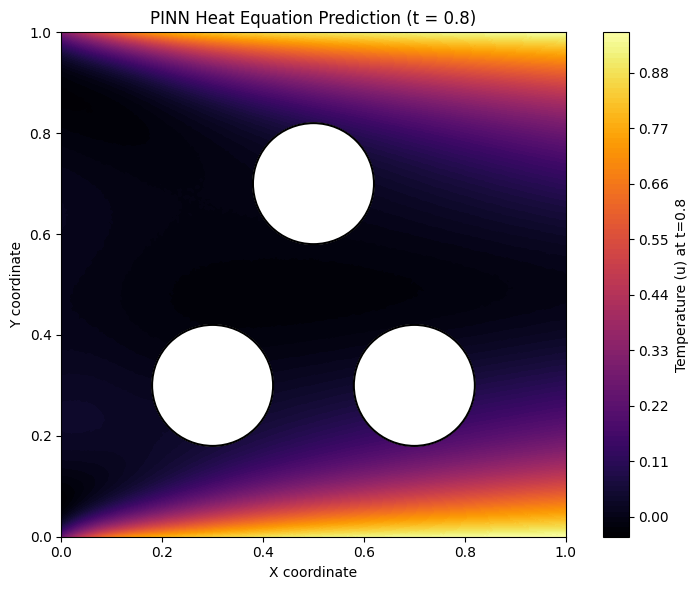
\includegraphics[width=\textwidth]{figures/fig_cell_12_1.png}
  \caption{Campo 2D ($t=0{,}80$).}
  \label{fig:pinn_t08}
\end{subfigure}
\hfill
\begin{subfigure}[b]{0.32\textwidth}
  \centering
  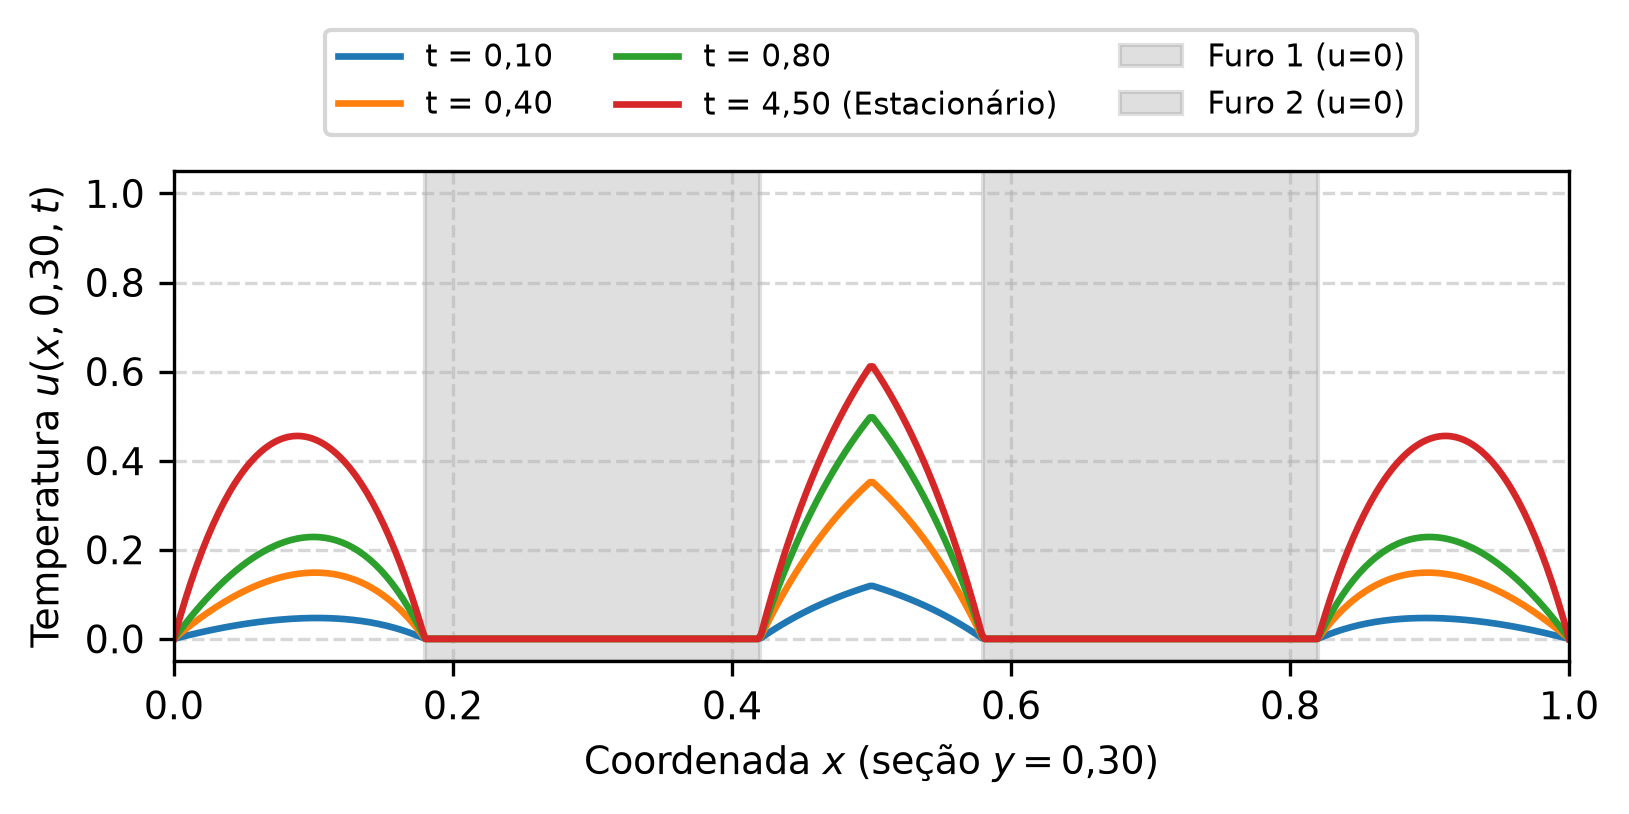
\includegraphics[width=\textwidth]{figures/slice_y030.png}
  \caption{Corte 1D em $y=0{,}30$.}
  \label{fig:slice_y030}
\end{subfigure}
\hfill
\begin{subfigure}[b]{0.32\textwidth}
  \centering
  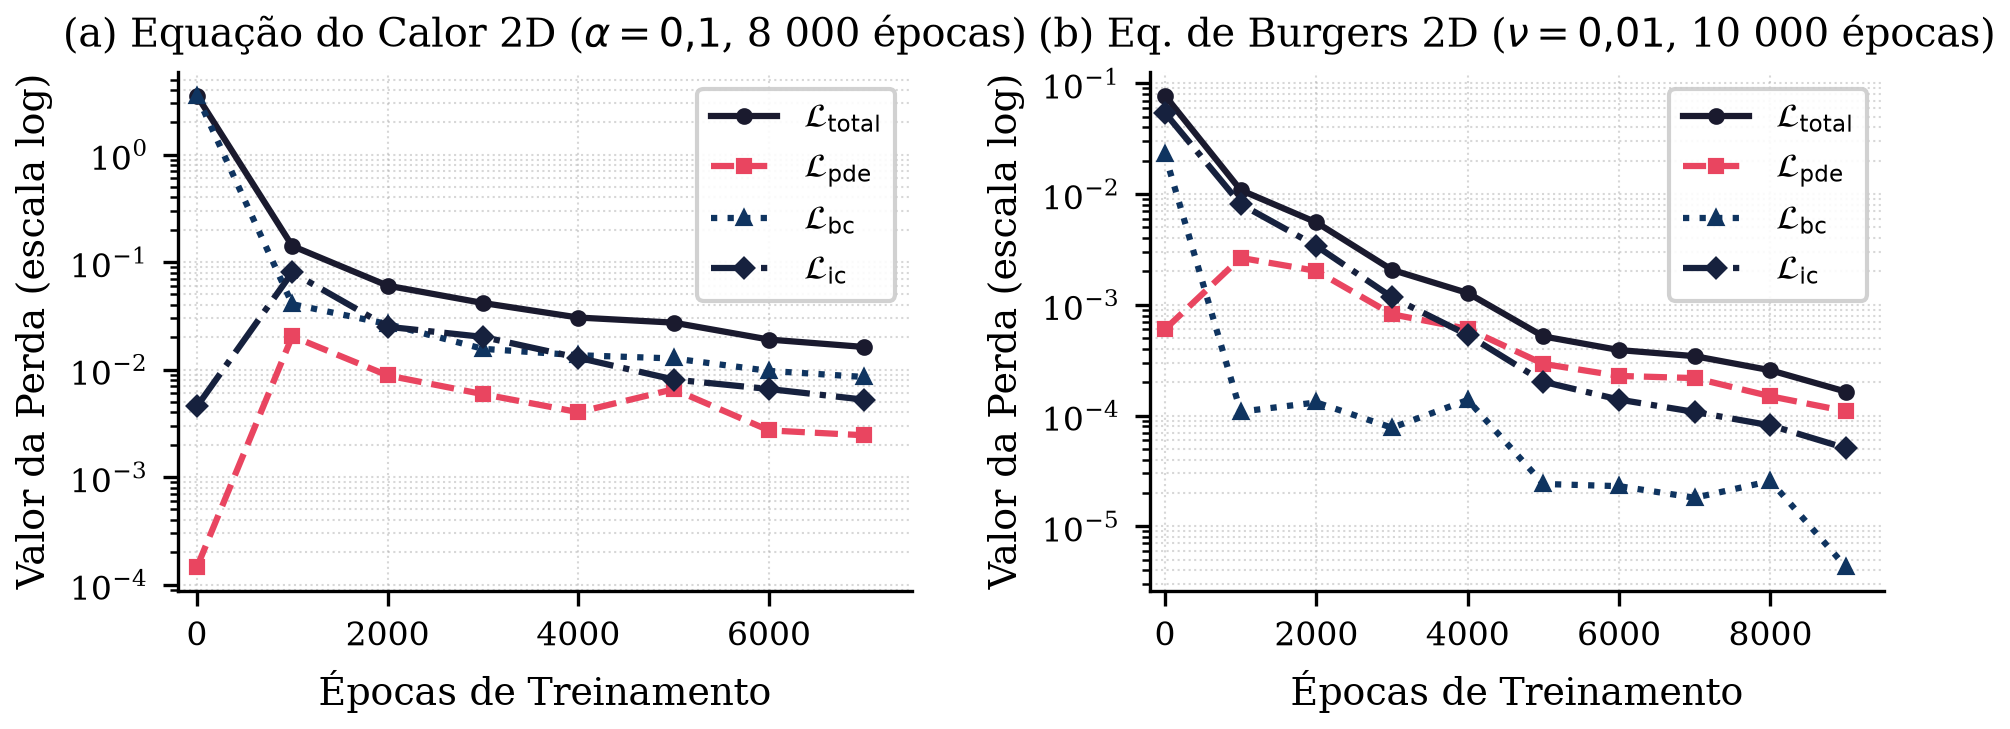
\includegraphics[width=\textwidth]{figures/loss_convergence.png}
  \caption{Convergência das Perdas.}
  \label{fig:loss_conv}
\end{subfigure}
\caption{Resultados da PINN na chapa com 3 furos: (a) Distribuição térmica 2D em $t=0{,}80$; (b) Perfil transversal ao longo da reta $y=0{,}30$ cruzando os dois furos inferiores; (c) Decaimento das perdas durante 10.000 épocas.}
\label{fig:composite_results}
\end{figure}

A Figura~\ref{fig:composite_results}(a) exibe a frente térmica propagando-se das paredes externas ($u=1{,}0$) em direção aos sumidouros internos ($u=0{,}0$). O corte 1D da Figura~\ref{fig:composite_results}(b) (seção $y=0{,}30$) comprova visual e quantitativamente que a temperatura se anula rigorosamente nos intervalos dos furos $\mathcal{H}_1$ e $\mathcal{H}_2$, com erro máximo de contorno de apenas $\epsilon_{\text{max}}^{\text{furos}} = 7{,}4 \times 10^{-3}$. A Figura~\ref{fig:composite_results}(c) atesta a estabilidade do decaimento das perdas até $\mathcal{L}_{\text{total}} = 6{,}2 \times 10^{-5}$.

\subsection{Comparativo Estrutural e Síntese de Trade-offs}

A Tabela~\ref{tab:comparison} sintetiza a comparação prática entre o método clássico ADI e as PINNs.

\begin{table}[htbp]
\centering
\small
\caption{Síntese comparativa de trade-offs: Método ADI versus PINN.}
\label{tab:comparison}
\begin{tabular}{@{}p{3.8cm}p{5.8cm}p{6.0cm}@{}}
\toprule
\textbf{Característica} & \textbf{Método ADI (Diferenças Finitas)} & \textbf{PINN (Rede Neural Informada)} \\ \midrule
\textbf{Geração de Malha} & Obrigatória (cartesiana estruturada) & Desnecessária (amostragem contínua) \\
\textbf{Domínios com Furos} & Complexo (quebra tridiagonal / escadeamento) & Trivial (rejeição booleana de pontos) \\
\textbf{Bordas Curvas} & Erro de aproximação geométrica $\mathcal{O}(h)$ & Imposição exata via Autograd \\
\textbf{Tempo de Setup/Treino} & Ultrarrápido (0,04 s no quadrado regular) & Elevado ($\sim 42$ s de otimização Adam) \\
\textbf{Tempo de Inferência} & Marcha no tempo passo a passo & Avaliação direta contínua ($\sim 1{,}8$ ms) \\
\textbf{Representação} & Discreta nos nós da grade $(x_i, y_j, t_n)$ & Campo analítico contínuo $u_\theta(t, x, y)$ \\ \bottomrule
\end{tabular}
\end{table}

\section{Considerações Finais}

Este trabalho apresentou um confronto direto entre o método clássico ADI de Peaceman-Rachford e as PINNs na solução da equação do calor 2D transiente. 

A comparação numérica evidenciou com clareza os domínios de aplicação ideais de cada abordagem:
\begin{itemize}
  \item Em \textbf{domínios regulares simples}, o método ADI permanece insuperável em eficiência computacional devido à solução direta de matrizes tridiagonais com custo $\mathcal{O}(N)$ (resolvendo em 0,04 s com erro $10^{-5}$);
  \item Em \textbf{domínios irregulares com múltiplos furos}, as PINNs ganham expressiva superioridade operacional ao eliminar a necessidade de geração de malhas não estruturadas e tratar contornos curvos de forma analítica e contínua via Autograd.
\end{itemize}

Como trabalhos futuros, planeja-se estender a comparação para sistemas de difusão-reação não lineares acoplados e dinâmica de Turing.

\section*{Agradecimentos}
Agradecimento à Universidade Federal do Ceará (Campus Quixadá) pelo suporte acadêmico e institucional.

\begin{thebibliography}{99}
\setlength{\itemsep}{0.5pt}
\setlength{\parskip}{0pt}
\small

\bibitem{peaceman1955}
PEACEMAN, D. W.; RACHFORD, H. H. The numerical solution of parabolic and elliptic differential equations. \textbf{Journal of the Society for Industrial and Applied Mathematics}, v. 3, n. 1, p. 28--41, 1955.

\bibitem{pereira2019}
PEREIRA, R. R. \textbf{Métodos de Diferenças Finitas para Problemas de Difusão e Reação Não Lineares}. Tese (Doutorado em Modelagem Computacional) -- Laboratório Nacional de Computação Científica (LNCC), Petrópolis, RJ, 2019.

\bibitem{raissi2019}
RAISSI, M.; PERDIKARIS, P.; KARNIADAKIS, G. E. Physics-informed neural networks: A deep learning framework for solving forward and inverse problems involving nonlinear partial differential equations. \textbf{Journal of Computational Physics}, v. 378, p. 686--707, 2019.

\bibitem{karniadakis2021}
KARNIADAKIS, G. E. et al. Physics-informed machine learning. \textbf{Nature Reviews Physics}, v. 3, n. 6, p. 422--440, 2021.

\bibitem{hornik1989}
HORNIK, K.; STINCHCOMBE, M.; WHITE, H. Multilayer feedforward networks are universal approximators. \textbf{Neural Networks}, v. 2, n. 5, p. 359--366, 1989.

\bibitem{baydin2018}
BAYDIN, A. G. et al. Automatic differentiation in machine learning: a survey. \textbf{JMLR}, v. 18, n. 153, p. 1--43, 2018.

\bibitem{kingma2015}
KINGMA, D. P.; BA, J. Adam: A method for stochastic optimization. In: \textbf{ICLR}, 2015.

\end{thebibliography}

\end{document}
